%-----------------------------------------------------------------------------------------------
\makeatletter
\immediate\write18{datelog > \jobname.info} % site script for $(date '+%Y-%m-%d %Hh%Mm%Ss')
\makeatother
%-----------------------------------------------------------------------------------------------
%-----------------------------------------------------------------------------------------------
\usetheme{Copenhagen}
\usepackage{beamercolorthemeUTF2}
\usefonttheme{serif}
%-----------------------------------------------------------------------------------------------
\usepackage[utf8]{inputenc}
\usepackage[greek,french,english,brazil]{babel} % last becomes the active one
\usepackage{pslatex}
\usepackage{amssymb,amsmath}
\usepackage{soul}
\usepackage[squaren,Gray,cdot]{SIunits}
\usepackage[nice]{nicefrac}
\usepackage{tikz}
\usepackage{amscd}
\usepackage{stmaryrd}
\usepackage{scalerel}
\usepackage{xspace}
%-----------------------------------------------------------------------------------------------


%-----------------------------------------------------------------------------------------------
%-----------------------------------------------------------------------------------------------
% Mathematical
%-----------------------------------------------------------------------------------------------
\newcommand{\vet}[1]{\underline{{#1}}}
\newcommand{\mat}[1]{\underline{\underline{{#1}}}}
\newcommand{\cub}[1]{\underline{\underline{\underline{{#1}}}}}
\newcommand{\eqdef}{{\ensuremath\stackrel{\text{\tiny def}}{=}}}
%-----------------------------------------------------------------------------------------------
% Linguistic
%-----------------------------------------------------------------------------------------------
\newcommand{\GRtxt}[1]{\begin{otherlanguage}{greek}{{#1}}\end{otherlanguage}}
\newcommand{\FRtxt}[1]{\begin{otherlanguage}{french}{{#1}}\end{otherlanguage}}
%-----------------------------------------------------------------------------------------------
% Presentation
%-----------------------------------------------------------------------------------------------
\newcommand{\BkgImgH}[1]{% Places an image centered on the slide background filling the height
    \usebackgroundtemplate{\parbox{\paperwidth}{%
        \vspace*{1sp}\centering\includegraphics[height=\paperheight]{{#1}}
}}}
\newcommand{\BkgImgW}[1]{% Places an image centered on the slide background filling the width
    \usebackgroundtemplate{\parbox{\paperwidth}{%
        \vspace*{1sp}\centering\includegraphics[width=\paperwidth]{{#1}}
}}}
\newcommand{\ArtEndH}[3]{% Transitions to plain image (last) slide: #1:prefix #2,#3:extensions
    \BkgImgH{root/../art/#1.#2}
    \frame<handout:0>[plain]{%
        \transdissolve\vspace*{72mm}\color{white}\scriptsize\bf\input{root/../art/#1.#3}}
    \usebackgroundtemplate{\mbox{~}}
}
\newcommand{\ArtEndW}[3]{% Transitions to plain image (last) slide: #1:prefix #2,#3:extensions
    \BkgImgW{root/../art/#1.#2}
    \frame<handout:0>[plain]{%
        \transdissolve\vspace*{72mm}\color{white}\scriptsize\bf\input{root/../art/#1.#3}}
    \usebackgroundtemplate{\mbox{~}}
}
\newcommand{\ImgColW}[3]{% Inserts a full-width image in a column
    \includegraphics[width=\columnwidth]{root/../art/#1.#2}\\[-0.5\baselineskip]
    \parbox{\columnwidth}{\tiny\hfill\scalebox{0.85}{\input{root/../art/#1.#3}}}
}
\newcommand{\txtpic}[1]{%
    \fcolorbox{lightgray}{white!90!black}{{#1}} 
}
%-----------------------------------------------------------------------------------------------


%-----------------------------------------------------------------------------------------------
\newcommand{\VPMS}{{\ensuremath V_{\mathrm{PMS}}}}
\newcommand{\VPMI}{{\ensuremath V_{\mathrm{PMI}}}}
%-----------------------------------------------------------------------------------------------
\title{C.01.01 -- Ciclo Otto de Tempo Finito de Adição de Calor}
\subtitle{FTHA -- Finite-Time Heat Addition Otto Engine Model}
\author{Prof.~C.~Naaktgeboren, PhD}
\date{{\scriptsize\tt%
    
\includegraphics[height=6.0mm]{root/00-res/cc/by-nc-nd-88x31.pdf}\\[\smallskipamount]
    https://github.com/CNThermSci/ApplThermSci\\
    Compiled on \input{\jobname.info}
}}
%-----------------------------------------------------------------------------------------------
\begin{document}
%-----------------------------------------------------------------------------------------------
\logo{%
    \parbox{158mm}{% There's a 1mm gap on each side of the 160mm x 90mm slide logo line
        
\includegraphics[height=6.5mm]{root/00-res/UTFPR/UTFPR-logo-A.pdf}\hfill%
        
\includegraphics[height=6.5mm]{root/00-res/logo/CNThermSci-logo-A.pdf}%
%   \parbox{126mm}{% There's a 1mm gap on each side of the 128mm x 96mm slide logo line
%       
\includegraphics[height=6.0mm]{root/00-res/UTFPR/UTFPR-logo-A.pdf}\hfill%
%       
\includegraphics[height=6.0mm]{root/00-res/logo/CNThermSci-logo-A.pdf}%
}} % Alpha logos
%-----------------------------------------------------------------------------------------------
\frame{\titlepage}
%-----------------------------------------------------------------------------------------------

%-----------------------------------------------------------------------------------------------
\frame{\tableofcontents}
%-----------------------------------------------------------------------------------------------

%-----------------------------------------------------------------------------------------------
\section{Introdução}
%-----------------------------------------------------------------------------------------------

%-----------------------------------------------------------------------------------------------
\subsection{Limitações do Ciclo Otto Ideal}
%-----------------------------------------------------------------------------------------------

    % !j 96 -i8
    %-------------------------------------------------------------------------------------------
    \begin{frame}{Melhorando o Ciclo Otto Ideal}\vspace*{-2em}
        \uncover<1->{O ciclo Otto \alert{ideal}, da termodinâmica aplicada:}
        \begin{columns}
        \column{0.50\textwidth}
        \begin{itemize}
            \item<2->  Assume todas as \alert{hipóteses padrão a ar};
            \item<8->  Assume entrada de calor \alert{isocórica};
            \item<9->  Possui parâmetros \alert{$r$} e \alert{$k$}, e
            \item<10-> Solução analítica, \alert{hip.~padrão a ar frio}:\\[\bigskipamount]
        \end{itemize}
        \begin{equation*}
            \uncover<12->{\alert{\eta_t = 1 - r^{1-k}}\quad\rightharpoondown}
        \end{equation*}%
        \vspace*{-1em}
        \begin{itemize}
            \item<13-> $\eta_t\!:\!\eta_t(r, k)$ \alert{apenas}!
        \end{itemize}
        \column{0.50\textwidth}
        \begin{itemize}
            \item<3->  Gás \alert{ideal};
            \item<4->  Processos \alert{internamente reversíveis};
            \item<5->  Entrada de \alert{calor} modela a combustão;
            \item<6->  Saída de \alert{calor} modela a exaustão;
            \item<7->  Modelo em \alert{ciclo fechado};
            \item<11-> Calores específicos \alert{constantes}.
        \end{itemize}
        \end{columns}
    \end{frame}
    %-------------------------------------------------------------------------------------------

    % !j 96 -i8
    %-------------------------------------------------------------------------------------------
    \begin{frame}{Desvios do ciclo Otto ideal---incluem, mas não limitados a:}\vspace*{-2em}
        \begin{center}
            \includegraphics[height=40mm,width=60mm]{%
                fig/P-V_diagram_deviations_to_Otto_cycle.pdf}\\
            \footnotesize  Diagrama  $P-V$  ilustrativo  de   perdas   por   (i)~combustão   não
                instantânea---verde,    (ii)~transferência    de     calor---vermelho---e     de
                (iii)~bombeamento---azul. Fonte: adaptado de Wikimedia Commons.
            {\tiny\tt https://upload.wikimedia.org/wikipedia/commons/6/6c/P-V\_diagram\_deviations\_to\_Otto\_cycle.svg.}
        \end{center}
    \end{frame}
    %-------------------------------------------------------------------------------------------

%-----------------------------------------------------------------------------------------------
\subsection{Proposta do Ciclo Otto FTHA}
%-----------------------------------------------------------------------------------------------

    % !j 96 -i8
    %-------------------------------------------------------------------------------------------
    \begin{frame}{Ciclo Otto padrão a ar de tempo finito de adição de calor---FTHA}\vspace*{-2em}
        \begin{itemize}
            \item<1->  Modela combustão (adição de calor) de forma \alert{não instantânea}:
            \begin{itemize}
                \item<2->  Interações \alert{simultâneas} de \alert{calor} e \alert{trabalho};
                \item<3->  Tempos de motor \alert{discretizados} em \alert{sub-processos};
                \item<4->  Elemento computacional: sub-processo \alert{localmente politrópico};
                \item<5->  \alert{Remoção} de calor permanece \alert{isocórica} (instantânea).
            \end{itemize}
            \item<6->  Mantém-se como modelo \alert{padrão a ar}:
            \begin{itemize}
                \item<7->  Transferência de calor para bloco inclui \alert{irreversibilidades};
                \item<8->  Perdas de bombeamento envolvem \alert{sistema e ciclo abertos}.
            \end{itemize}
            \item<9->  Mantém-se como modelo de \alert{substância pura}:
            \begin{itemize}
                \item<10-> Evita \alert{combustão e equilíbrio químico};
                \item<11-> Evita modelagem termodinâmica de \alert{misturas reativas}.
            \end{itemize}
        \end{itemize}
    \end{frame}
    %-------------------------------------------------------------------------------------------

    % !j 96 -i8
    %-------------------------------------------------------------------------------------------
    \begin{frame}{Ciclo Otto padrão a ar de tempo finito de adição de calor---FTHA}\vspace*{-2em}
        \begin{itemize}
            \item<1->  Inclui todos os parâmetros do \alert{ciclo Otto ideal}:
            \begin{itemize}
                \item<2->  \alert{Razão de compressão} do motor;
                \item<3->  \alert{Calores específicos} do fluido de trabalho.
            \end{itemize}
            \item<4->  Inclui parâmetros \alert{construtivos} do \alert{motor}:
            \begin{itemize}
                \item<5->  Conjunto \alert{pistão-cilindro};
                \item<6->  Mecanismo \alert{biela-manivela}.
            \end{itemize}
            \item<7->  Inclui parâmetros \alert{operacionais} do \alert{motor}:
            \begin{itemize}
                \item<8->  \alert{Velocidade angular} (rotação);
                \item<9->  Ângulo de \alert{ignição} e
                \item<10-> \alert{Duração da combustão}.
            \end{itemize}
        \end{itemize}
    \end{frame}
    %-------------------------------------------------------------------------------------------

%-----------------------------------------------------------------------------------------------
\section{Modelagem FTHA}
%-----------------------------------------------------------------------------------------------

%-----------------------------------------------------------------------------------------------
\subsection{Modelagem do Motor}
%-----------------------------------------------------------------------------------------------

    % !j 96 -i8
    %-------------------------------------------------------------------------------------------
    \begin{frame}{Parâmetros do mecanismo}\vspace*{-2em}
        \begin{columns}
        \column{0.60\textwidth}
        \begin{itemize}
            \item<1-> \alert{Diâmetro} do pistão/cilindro, \alert{$D$};
            \item<2-> \alert{Raio} da manivela, \alert{$R$};
            \item<3-> \alert{Curso} do pistão, \alert{$S = 2R$};
            \item<4-> \alert{Comprimento} da biela, \alert{$L$};
            \item<5-> \alert{Volume} morto (do PMS), \alert{$\VPMS$};
            \item<6-> \alert{Volume} máximo (do PMI), \alert{$\VPMI$};
            \item<7-> \alert{Razão de compressão}, \alert{$r = \dfrac{\VPMS}{\VPMI}$}.
        \end{itemize}
        \column{0.40\textwidth}
        \begin{center}
            \uncover<1->{\vspace*{-5mm}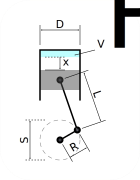
\includegraphics[height=70.0mm]{fig/FTHAEngine01.pdf}}
        \end{center}
        \end{columns}
    \end{frame}
    %-------------------------------------------------------------------------------------------

    % !j 96 -i8
    %-------------------------------------------------------------------------------------------
    \begin{frame}{Parâmetros do mecanismo}\vspace*{-2em}
        \begin{columns}
        \column{0.60\textwidth}
        \begin{itemize}
            \item<1-> \alert{Posição} do pistão (rel.~PMS), \alert{$x$};
            \item<2-> \alert{Ângulo} do virabrequim (rel.~PMS), \alert{$\alpha$};
            \item<3-> \alert{Volume} instantâneo, \alert{$V$};
        \end{itemize}
        \begin{align}
            \uncover<4->{
            x(\alpha)   &= L\left(1 - \sqrt{1 - \frac{R^2}{L^2}\sin^2\alpha}\right)
                        +  R(1 - \cos\alpha) \nonumber\\}
            \uncover<5->{
            V(\alpha)   &= \frac{\pi x(\alpha)}{4}D^2 + \VPMS\quad\rightharpoondown\quad
                        v(\alpha) = \frac{V(\alpha)}{m_0} \nonumber}
        \end{align}
        \column{0.40\textwidth}
        \begin{center}
            \uncover<1->{\vspace*{-5mm}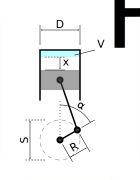
\includegraphics[height=70.0mm]{fig/FTHAEngine02.pdf}}
        \end{center}
        \end{columns}
    \end{frame}
    %-------------------------------------------------------------------------------------------

    % !j 96 -i8
    %-------------------------------------------------------------------------------------------
    \begin{frame}{Parâmetros de tempo do motor}\vspace*{-2em}
        \begin{columns}
        \column{0.60\textwidth}
        \vspace*{-1.0em}\begin{itemize}
            \item<1-> \alert{Ângulo} de ignição (rel.~PMS), \alert{$\theta$};
            \item<2-> \alert{Duração} da combustão, \alert{$\Delta t_c$};
            \item<3-> \alert{Velocidade angular}, \alert{$\omega \equiv \dfrac{d\alpha}{dt} =
                2\pi N/60$};
            \item<4-> ``\alert{Duração angular}'' da combustão, \alert{$\delta = \omega\Delta t_c$};
                \\[\medskipamount]
            \item<5-> Casos de \alert{$\omega$ constante}---discretização em $\alpha$:
            \begin{itemize}
                \item<5-> Intervalo de simulação: \alert{$-\pi \leqslant \alpha \leqslant +\pi$};
                \item<6-> Intervalo de adição de calor: \alert{$\theta \leqslant \alpha \leqslant
                    \theta+\delta$}.
                \item<7-> \alert{$\alpha_i = -\pi + i\Delta\alpha$}, $i \in \mathbb{N}$,
                          \alert{$0 \leqslant i \leqslant 2I$}, with
                \item<8-> \alert{$\Delta\alpha = \pi/I$},
                          \alert{$I \in \mathbb{N}^*$}.
                    \\[\medskipamount]
            \end{itemize}
            \item<9-> Casos de \alert{$\omega$ variável}---discretização em $t$.
        \end{itemize}
        \column{0.40\textwidth}
        \begin{center}
            \uncover<1->{\vspace*{-5mm}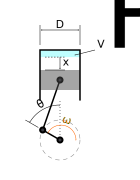
\includegraphics[height=70.0mm]{fig/FTHAEngine03.pdf}}
        \end{center}
        \end{columns}
    \end{frame}
    %-------------------------------------------------------------------------------------------

%-----------------------------------------------------------------------------------------------
\subsection{Modelagem do Ciclo}
%-----------------------------------------------------------------------------------------------

    % !j 96 -i8
    %-------------------------------------------------------------------------------------------
    \begin{frame}{Modelo de Adição de Calor, $q(\alpha)$}\vspace*{-2em}
        \begin{columns}
        \column{0.50\textwidth}
        \vspace*{-1.0ex}\begin{align}
            \uncover<1->{
            q(\alpha)   &= q_{ent} \cdot y(\alpha),\quad\mbox{com}\nonumber\\
            }
            \uncover<2->{
            \alert{y(\alpha)}   &\alert{=
            \begin{cases}
                0           & \mbox{para }\alpha < \theta,\\
                g(\alpha)   & \mbox{para }\theta \leqslant \alpha \leqslant \theta+\delta,\\
                1           & \mbox{para }\alpha > \theta+\delta.
            \end{cases}}\nonumber
            }
        \end{align}
        \vspace*{-3.0ex}\begin{itemize}
            \item<3-> \alert{$g(\alpha)$} modela o \alert{histórico} da ad.~de calor:
                \\[\smallskipamount]
            \begin{itemize}
                \item<4-> \alert{$g(\theta) = 0$} e \alert{$g(\theta+\delta) = 1$};
                    \\[\smallskipamount]
                \item<5-> \alert{Função} $g(\alpha)$ deve ser \alert{monotônica};
                    \\[\smallskipamount]
                \item<6-> $g(\alpha)$ pode basear-se em \alert{experimentos};
                    \\[\smallskipamount]
                \item<7-> Lit.:~\alert{$g(\alpha) = \frac{1}{2}-\frac{1}{2} \cos \bigl(
                    \frac{\pi}{\delta} (\alpha - \theta) \bigr)$}.
            \end{itemize}
        \end{itemize}
        \column{0.50\textwidth}
        \begin{center}
            \uncover<2->{\vspace*{-5mm}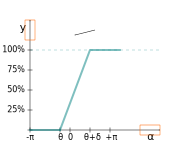
\includegraphics[height=70.0mm]{fig/FTHATiming01.pdf}}
        \end{center}
        \end{columns}
    \end{frame}
    %-------------------------------------------------------------------------------------------

    % !j 96 -i8
    %-------------------------------------------------------------------------------------------
    \begin{frame}{Equações Termodinâmicas}\vspace*{-2em}
        \uncover<1->{No $i$-ésimo (sub-)processo politrópico:}
        \begin{itemize}
            \item<2-> O sistema evolui do \alert{estado-$i$} para o \alert{estado-$(i+1)$}.
            \item<3-> \alert{Propriedades} $P_i$, $T_i$, $v_i$, $u_i$, etc., definidas nos
                \alert{estados} -$i$ e -$(i+1)$.
            \item<4-> \alert{Interações} do $i$-ésimo \alert{processo} são $q_i$ e $w_i$.
                \\[\bigskipamount]
        \end{itemize}
        \uncover<5->{Balanço de energia de processo:}
        \vspace*{-0.7em}\begin{align}
            \uncover<6->{q_i + w_i &= \Delta u_i = u_{i+1} - u_i}
            \uncover<7->{\quad\rightharpoondown\nonumber\\}
            \uncover<8->{\alert{u_{i+1}} &\alert{= u_i + q_i + w_i},\quad\mbox{com,}\nonumber}
        \end{align}
    \end{frame}
    %-------------------------------------------------------------------------------------------

    % !j 96 -i8
    %-------------------------------------------------------------------------------------------
    \begin{frame}{Equações Termodinâmicas}\vspace*{-2em}
        \begin{align}
            \uncover<1->{q_i &= q_{ent} \cdot (y_{i+1} - y_i)}
            \uncover<2->{\quad\rightharpoondown\nonumber\\[\medskipamount]}
            \uncover<3->{\alert{q_i} &\alert{= q_{ent} \cdot [y(\alpha_{i+1}) - y(\alpha_i)]},}
            \uncover<3->{\quad\mbox{e}\nonumber\\[\medskipamount]}
            \uncover<4->{w_i &= \int_{v_i}^{v_{i+1}}(P_iv_i^{n_i})v^{-n_i}\,dv,}
            \uncover<5->{\quad\rightharpoondown\nonumber\\[\medskipamount]}
            \uncover<6->{\alert{w_i} &\alert{= \begin{cases}
                \dfrac{P_i}{1-n_i}\left(v_i - \dfrac{v_i^{n_i}}{v_{i+1}^{n_i-1}}\right),\quad &
                \mbox{para }n_i \neq 1,\\[\bigskipamount]
                P_iv_i\ln\dfrac{v_i}{v_{i+1}}, &
                \mbox{para }n_i = 1,\\[\bigskipamount]
                0 & \mbox{para }v_i \approx v_{i+1} \quad\rightharpoondown\quad
                |v_i - v_{i+1}| \leqslant \epsilon_v.
            \end{cases}}\nonumber}
        \end{align}
    \end{frame}
    %-------------------------------------------------------------------------------------------

%-----------------------------------------------------------------------------------------------
\subsection{Procedimento de Solução}
%-----------------------------------------------------------------------------------------------

    % !j 96 -i8
    %-------------------------------------------------------------------------------------------
    \begin{frame}{Solução de Sub-Processo}\vspace*{-2em}
        \begin{cnj}[de consistência termodinâmica]
            Para  uma  dada  interação  de  calor,  $q_i$,  existe  um   \alert{único   expoente
            politrópico,  $n_i$},  tal  que  o  processo   politrópico   $Pv^{n_i}   =   C_i   =
            \mathrm{const.}$, aplicado entre estados ($i$) e ($i+1$) resulta em uma interação de
            trabalho, $w_i$, e em uma variação de energia interna, $\Delta u_i = u_{i+1} - u_i$,
            que é \alert{termodinamicamente consistente} com  a  \alert{equação  $P$-$v$-$T$  de
            estado} da substância de trabalho em ambos estados finais e que  também  satisfaz  o
            \alert{balanço de energia} do processo.
        \end{cnj}
        \vspace*{\smallskipamount}\uncover<2->{$\rightharpoondown$          Processo          de
        \alert{estimativa} $(n_i^0)$ e $j$-ésima \alert{correção} $(n_i^j)$ até a convergência.}
        \vspace*{\smallskipamount}\uncover<3->{Tolerâncias  de   convergência   $\epsilon_w$   e
        $\epsilon_u$.}
    \end{frame}
    %-------------------------------------------------------------------------------------------

    % !j 96 -i8
    %-------------------------------------------------------------------------------------------
    \begin{frame}{Algoritmo de Inicialização}\vspace*{-2em}
        \small
        \begin{tcolorbox}[colback=uyel!15!white]\begin{algorithmic}[1]
            \REQUIRE{Parâmetros do motor: $\{\omega, D, L, R, \VPMS,$ e $V_{du}\}$;}
            \REQUIRE{Ângulos $\theta$ e $\delta$ (via $\Delta t_c$);}
            \REQUIRE{Refinamento da discretização, $I$;}
            \REQUIRE{Estado inicial $(P_0, T_0)$ e modelo de substância;}
            \REQUIRE{Função $g(\alpha)$ e $q_{ent}$;}
            \REQUIRE{Tolerâncias de convergência $\epsilon_v$, $\epsilon_w$ e $\epsilon_u$.}
            \STATE{Inicializa todas quant.~com índice $i$ como vetores vazios:
                $\alpha_i$, $v_i$, $q_i$, $w_i$, $n_i$, $P_i$, $T_i$, and $u_i$;}
            \STATE{Calcula $\Delta\alpha = \pi/I$ e todos $\alpha_i = -\pi + i\Delta\alpha$;}
            \STATE{$v_0 \leftarrow $ volume específico, de $(P_0, T_0)$ e equação de estado;}
            \STATE{$m \leftarrow V_0/v_0$;}
            \STATE{Calcula todos $v_i = V(\alpha_i)/m$;}
            \STATE{$i \leftarrow 0$;}
        \end{algorithmic}\end{tcolorbox}
    \end{frame}
    %-------------------------------------------------------------------------------------------

    % !j 96 -i8
    %-------------------------------------------------------------------------------------------
    \begin{frame}{Algoritmo de Laço do Ciclo}\vspace*{-2em}
        \small
        \begin{tcolorbox}[colback=uyel!15!white]\begin{algorithmic}[1]
            \FOR{$i=0$ até $2I$}
                \STATE{Calcula $q_i = q_{ent} \cdot [y(\alpha_{i+1}) - y(\alpha_i)]$;}
                \STATE{Resolve para $w_i$, $n_i$, $u_{i+1}$, $P_{i+1}$ e $T_{i+1}$
                    via algoritmo de solução de sub-processo;}
            \ENDFOR
            \STATE{$i \leftarrow i+1$;}
            \STATE{$q_i \leftarrow u_0 - u_i$;}
            \STATE{$w_i \leftarrow 0$;}
            \STATE{Estado-($i$) = Estado-0;}
                \COMMENT{Para todas as funções de estado rastreadas}
        \end{algorithmic}\end{tcolorbox}
    \end{frame}
    %-------------------------------------------------------------------------------------------

    % !j 96 -i8
    %-------------------------------------------------------------------------------------------
    \begin{frame}{Algoritmo de Finalização}\vspace*{-2em}
        \small
        \begin{tcolorbox}[colback=uyel!15!white]\begin{algorithmic}[1]
            \STATE{$w_{ent} \leftarrow \sum w_i \geqslant 0$;}
                \COMMENT{Trabalho que entra no sistema}
            \STATE{$w_{out} \leftarrow - \sum w_i < 0$;}
                \COMMENT{Trabalho realizado pela sistema}
            \STATE{$w_{net} \leftarrow w_{out} - w_{ent}$;}
                \COMMENT{Trabalho líquido realizado pelo sistema}
            \STATE{$q_{ent} \leftarrow \sum q_i \geqslant 0$;}
                \COMMENT{Calor que entra no sistema}
            \STATE{$q_{rej} \leftarrow - \sum q_i < 0$;}
                \COMMENT{Calor rejeitado pelo sistema}
            \STATE{$\eta_t  \leftarrow w_{net} / q_{ent}$;}
                \COMMENT{Eficiência térmica}
            \STATE{$r_{bw}  \leftarrow w_{ent} / w_{out}$;}
                \COMMENT{Fração de consumo de trabalho}
            \STATE{MEP     $\leftarrow w_{net} / (V_{du} / m)$;}
                \COMMENT{Pressão média efetiva}
            \STATE{Salva dados da simulação para o pós-processamento (relatório).}
        \end{algorithmic}\end{tcolorbox}
    \end{frame}
    %-------------------------------------------------------------------------------------------

%-----------------------------------------------------------------------------------------------
\section{Tópicos de Leitura}
%-----------------------------------------------------------------------------------------------

    %------------------------------------------------------------------------------------------
    \begin{frame}[allowframebreaks]{Tópicos de Leitura}
        \begin{thebibliography}{Çengel, Y.~A., 2013}
            \bibitem[Çengel, Y.~A., 2013]{2013-CengelYA+BolesMA-AMGH}
                Çengel, Y.~A. e Boles, M.~A.
                \newblock{%
                    {\em Termodinâmica $7^\mathrm{a}\!$ Edição\/}.
                    \alert{Seções~9--3 a 9--5.}
                }
                \newblock{\footnotesize AMGH. Porto Alegre. ISBN 978-85-8055-200-3.}
            \bibitem[Naaktgeboren, C., 2016]{2017-NaaktgeborenC-IntJMechEngEduc}
                Naaktgeboren, C.
                \newblock{%
                    {\em An air-standard finite-time heat addition Otto engine model\/}.
                }
                \newblock{\alert{Int.~J.~Mech.~Eng.~Educ. 45 (2), 2017.}}
                \newblock{\footnotesize DOI 10.1177/0306419016689447.}
        \end{thebibliography}
    \end{frame}
    %------------------------------------------------------------------------------------------

    % Finishes with stunning image, with credit
    \ArtEndW{horizon-768759_1280}{jpg}{txt}

%-----------------------------------------------------------------------------------------------
\end{document}
%-----------------------------------------------------------------------------------------------

